
\section{Experiment}

\begin{figure}[t]
  \centering
  
  \includegraphics[width=1.0 \textwidth]{fig/fig_main_result.pdf} 
  \vspace{-0.6cm}
  
  \caption{\textbf{Qualitative results of COVE.} COVE can effectively handle various types of prompts, generating high-quality videos. For both global editing (e.g., style transferring and background editing) and local editing (e.g., modifying the appearance of the subject), COVE demonstrates outstanding performance. Results are best-viewed zoomed-in.}
  
  \label{fig:ours_main}
  
\end{figure}

\subsection{Experimental Setup}

In the experiment, we adopt Stable Diffusion (SD) 2.1 from the official Huggingface repository for COVE, employing 100 steps of DDIM inversion and 50 steps of denoising. To extract the diffusion feature, the noise of the specific timestep $t=261$ is added to each frame of the source video following \cite{tang2023emergent}. The feature is then extracted from the intermediate layer of the 2D Unet decoder during a single step of denoising. The window size $l$ is set to 9 for correspondence calculation, and $k$ is set to 3 for correspondence-guided attention. The merge ratio for token merging is 50\%. For both qualitative and quantitative evaluation, we select 23 videos from social media platforms such as TikTok and other publicly available sources \cite{pexels, pixabay}. Among these 23 videos, 3 videos have a length of 10 frames, 15 videos have a length of 20 frames, and 5 videos have a length of 32 frames. The experiments are conducted on a single RTX 3090 GPU for our method unless otherwise specified.  
We compare COVE with 5 baseline methods: FateZero \cite{qi2023fatezero}, TokenFlow \cite{geyer2023tokenflow}, FLATTEN \cite{cong2023flatten}, FRESCO \cite{yang2024fresco} and RAVE \cite{kara2023rave}. For all of these baseline methods, we follow the default settings from their official Github repositories. The more detailed experimental settings of our method are provided in \Cref{sec:app_set}.









\subsection{Qualitative Results}

We evaluate COVE on various videos under different types of prompts including both global and local editing (\Cref{fig:ours_main}). Global editing mainly involves background editing and style transferring. For background editing, COVE can modify the background while keeping the subject of the video unchanged (e.g. Third row, first column. \enquote{\texttt{a car driving in milky way}}). For style transfer, COVE can effectively modify the global style of the source video according to the prompt (e.g. Third row, second column. \enquote{\texttt{Van Gogh style}}). Our prompts for local editing include changing the subject of the video to another one (e.g. Third row, third column. \enquote{\texttt{A cute raccoon}}) and making local edits to the subject (e.g. fifth row, third column. \enquote{\texttt{A sorrow woman}}). For all of these editing tasks, COVE demonstrates outstanding performance, generating frames with high visual quality while successfully preserving temporal consistency. We also compare COVE with a wide range of state-of-the-art video editing methods (\Cref{fig:compare}). The experimental results illustrate that COVE effectively edits the video with high quality, significantly outperforming the previous methods.

\begin{figure}
  \centering
  
  \includegraphics[width=1.0 \textwidth]{fig/fig_baseline_3.pdf} 
  \vspace{-0.5cm}
    \caption{\textbf{Qualitative comparison of COVE and various state-of-the-art methods.} Our method outperforms previous methods across a wide range of source videos and editing prompts, demonstrating superior visual quality and temporal consistency. Results are best-viewed zoomed-in.}
    \vspace{-0.6cm}
    \label{fig:compare}
\end{figure}


\subsection{Quantitative Results}

For quantitative comparison, we follow the metrics proposed in VBench \cite{huang2023vbench}, including Subject Consistency, Motion Smoothness, Aesthetic Quality, and Imaging Quality. Among them, Subject Consistency assesses whether the subject (e.g., a person) remains consistent throughout the whole video by calculating the similarity of DINO \cite{caron2021emerging} feature across frames. Motion Smoothness utilizes the motion priors of the video frame interpolation
model \cite{li2023amt} to evaluate the smoothness of the motion in the generated video. Aesthetic Quality uses the LAION aesthetic predictor \cite{LAIONaes} to assess the artistic and beauty value perceived by humans on each frame. Imaging Quality evaluates the degree of distortion in the generated frames (e.g., blurring, flickering) through the MUSIQ \cite{ke2021musiq} image quality predictor. 
Each video undergoes editing with 3 global prompts (such as style transferring, background editing, etc.) and 2 local prompts (such as editing the appearance of the subject in the video), generating a total of 115 text-video pairs. For each metric, we report the average score of these 115 videos. We further conducted a user study with 45 participants following \cite{yang2024fresco}. Participants are required to choose the most preferable results among these methods. The result is shown in \Cref{tab:compare}.
Among various methods, COVE achieves outstanding performance in both qualitative metrics and user studies, further demonstrating its superiority.


\noindent 

\begin{minipage}{0.54\textwidth}
    \vspace{2.5mm}
    \resizebox{\linewidth}{!}{
    \begin{tabular}{c|cccccc}
    \toprule  
    &Subject          & Motion        &Aesthetic      & Imaging  &User\\
    &Consistency        & Smoothness    &Quality        & Quality &Study\\
    \midrule
    FateZero \cite{qi2023fatezero}     & 0.9622            & 0.9547        & 0.6258        &0.6951  & 7.4\%\\
    TokenFlow \cite{geyer2023tokenflow}      & 0.9513            & 0.9803        & 0.6904        &0.7354 & 13.0\% \\
    FLATTEN \cite{cong2023flatten}        & 0.9617            & 0.9622        & 0.6544        &0.7155 & 14.8\% \\
    FRESCO  \cite{yang2024fresco}        & 0.9358            & 0.9737        & 0.6582        &0.6331 & 9.2\% \\
    RAVE    \cite{kara2023rave}        & 0.9518            & 0.9732        & 0.6369        &0.7355  & 11.1\% \\
   
    \textbf{COVE (Ours)}   & \textbf{0.9731}            & \textbf{0.9892}        & \textbf{0.7122 }       &\textbf{0.7441} & \textbf{44.5\%} \\
    \bottomrule
    \end{tabular}
    }
    \vspace{-1mm}
    
    \captionof{table}{\textbf{Quantitative comparison} among COVE and a wide range of state-of-the-art video editing methods. The evaluation metrics\cite{huang2023vbench} can effectively reflect the temporal consistency and frame quality of generated videos. COVE illustrates superior performance in both keeping the temporal consistency and generating frames with high quality in edited videos.} 
    \label{tab:compare}
    \vspace{5mm}


    \hspace{2mm}
    \resizebox{0.95\linewidth}{!}{
    \begin{tabular}{c|ccccc}
    \toprule  
    &Subject            & Motion        &Aesthetic      & Imaging  \\
    &Consistency        & Smoothness    &Quality        & Quality \\
    \midrule
    w/o     & 0.9431            & 0.9049        & 0.6913        &0.7132  \\
    $K=1$   & 0.9637            & 0.9817        & 0.6979        &0.7148  \\
    $K=3$   & {0.9731}            & \textbf{0.9892}        & 0.7122        &\textbf{0.7441}  \\
    $K=5$   & \textbf{0.9745}            & 0.9886       & \textbf{0.7167 }       &{0.7429}  \\
    \bottomrule
  \end{tabular}
    }
    \vspace{-0.2mm}
    \captionof{table}{\textbf{Ablation study on the value of $K$ in correspondence-guided attention.} w / o means without correspondence-guided attention in Unet. When $K=3$ the quality of the video is the best. } 
    \label{tab:ablate}
\end{minipage}
\hspace{2mm}
\begin{minipage}{0.44\textwidth}
    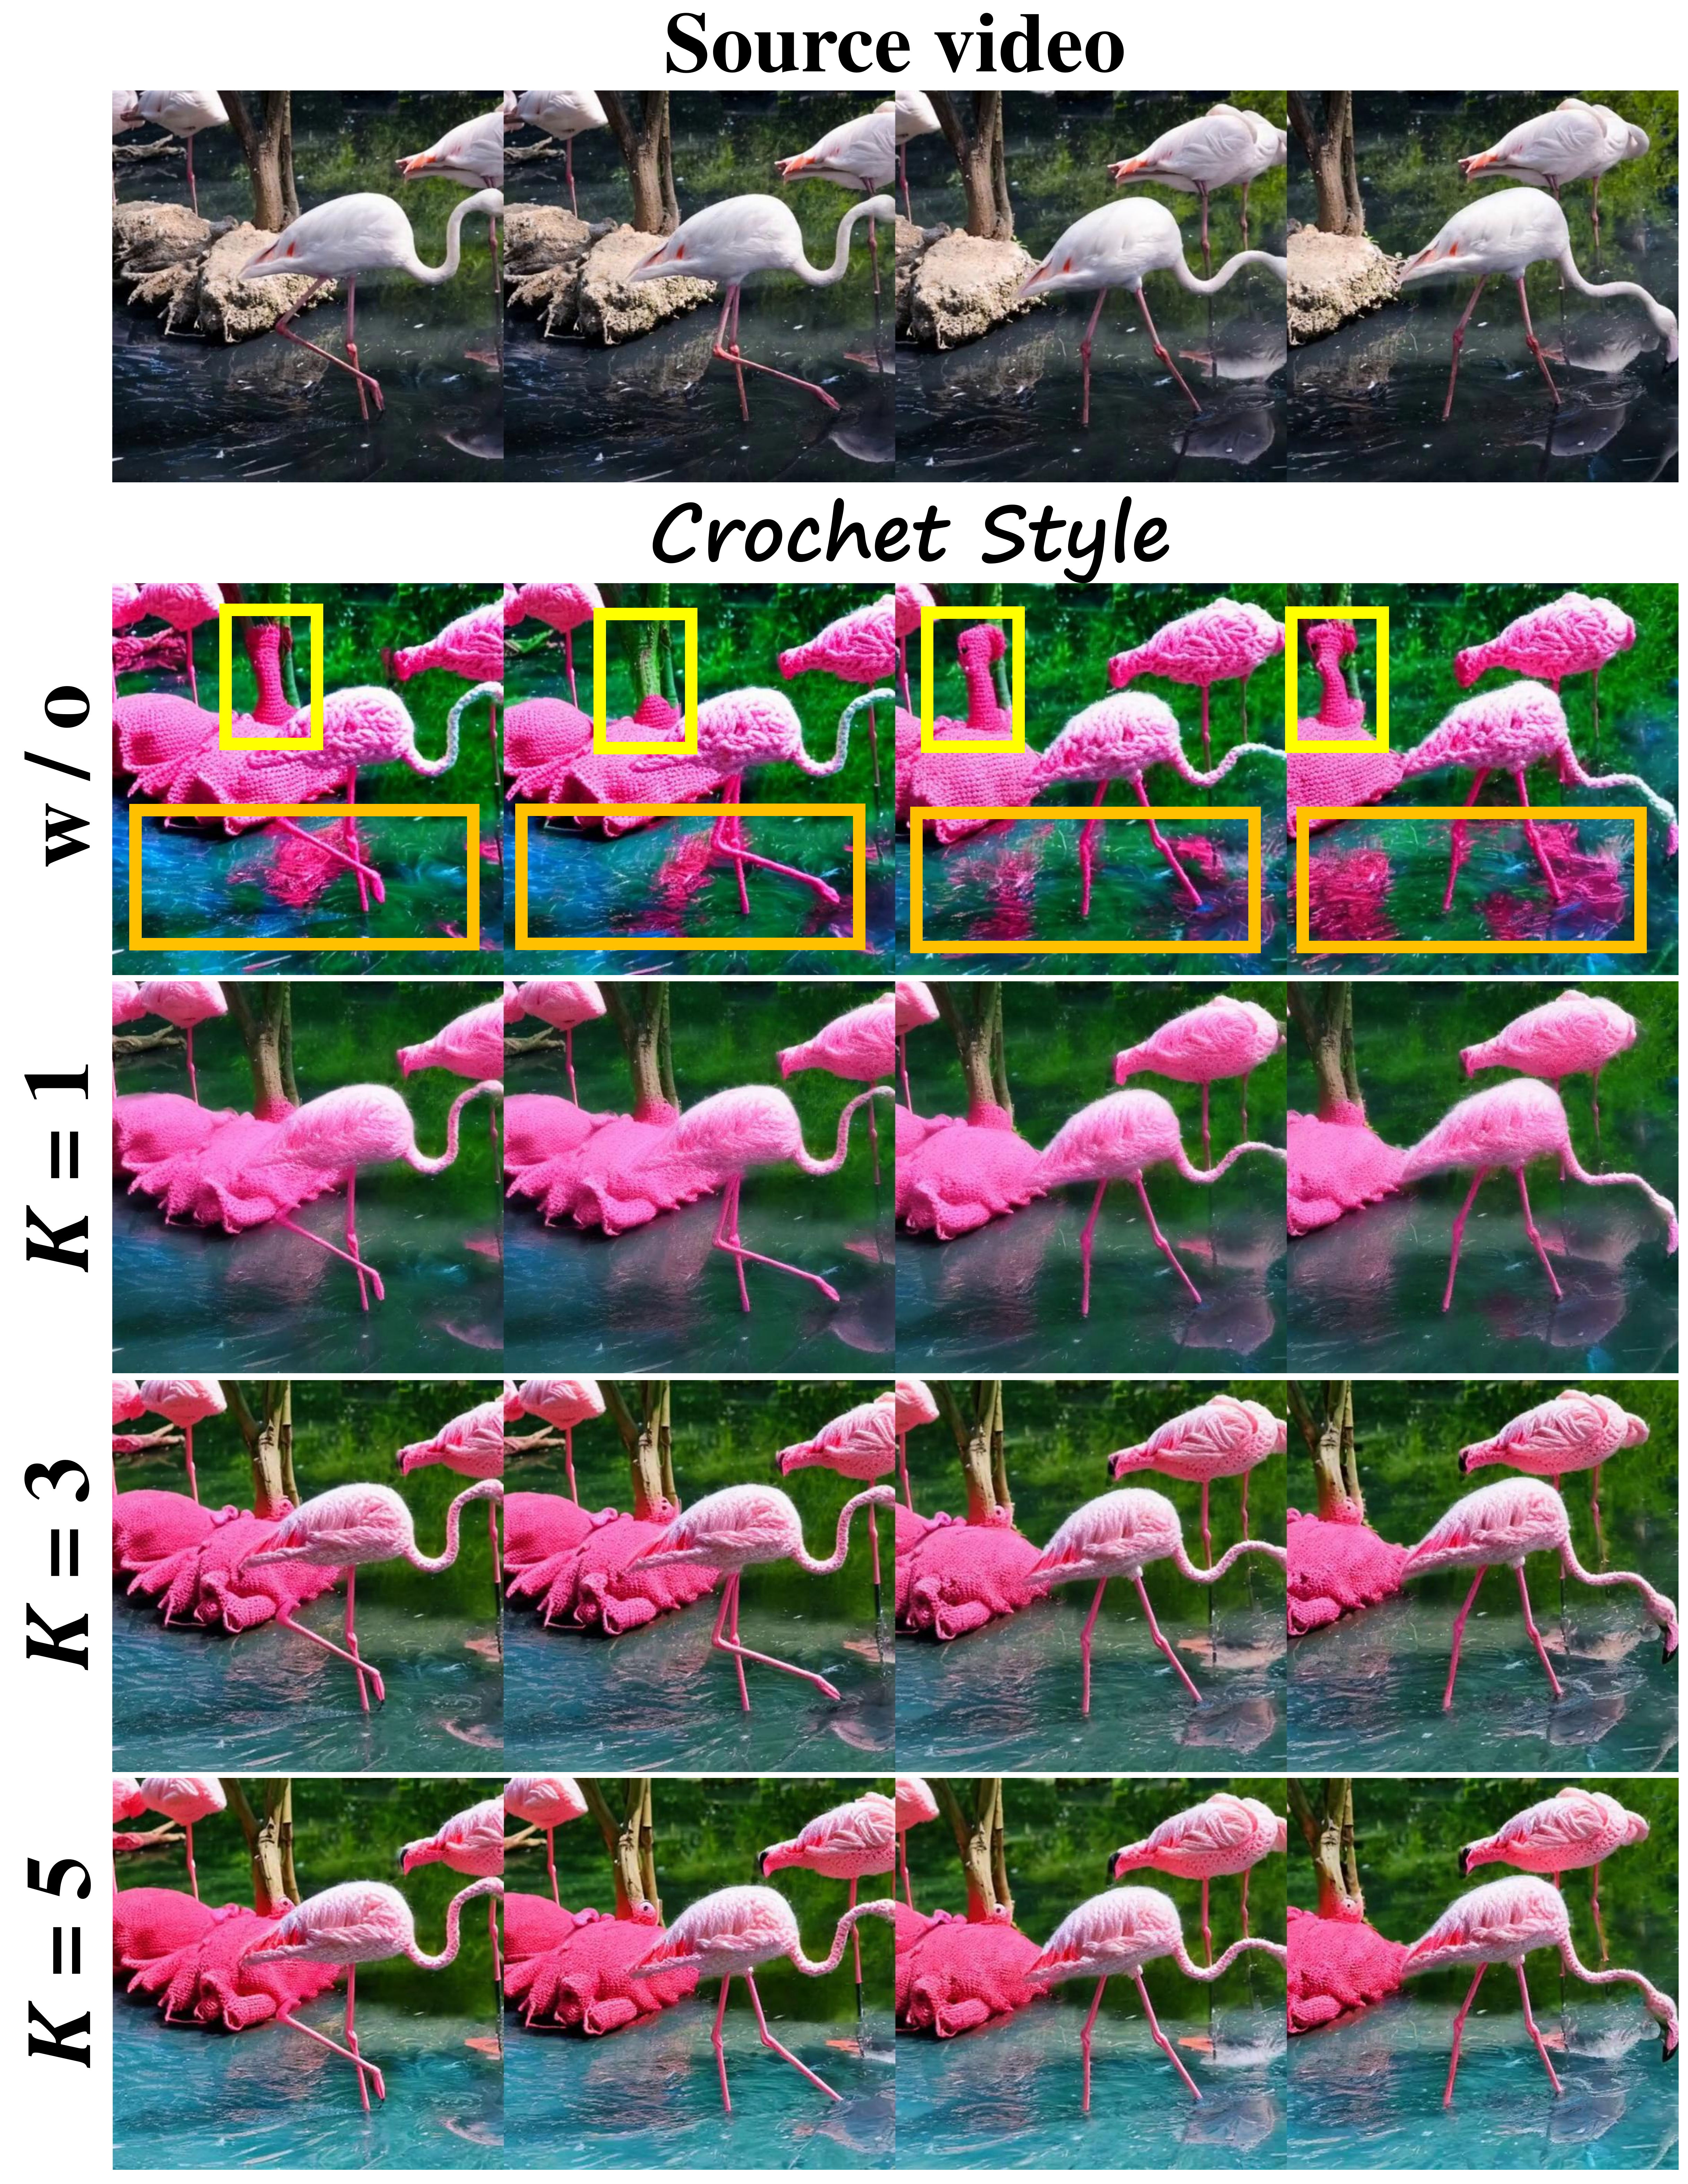
\includegraphics[width=\linewidth]{fig/fig_abla.pdf} 
    \vspace{-3mm}
    \captionof{figure}{Ablation study about the correspondence-guided attention and the value of $K$.  w / o means do not apply correspondence-guided attention.} 
    \label{fig:ablate}
\end{minipage}%






\subsection{Ablation Study}

We conduct an ablation study to illustrate the effectiveness of the \textbf{Correspondence-guided attention} and the number of tokens selected in each frame (i.e., the value of $K$). The experimental results (\Cref{tab:ablate} and \Cref{fig:ablate}) illustrate that without correspondence-guided attention, the edited video exhibits obvious temporal inconsistency and flickering effects (which is marked in \textcolor[RGB]{200,200,0}{\textbf{yellow}} and \textcolor{orange}{\textbf{orange}} boxes in \Cref{fig:ablate}), thus severely impairing the visual quality. As $K$ increases from 1 to 3, the generated video contains more fine-grained details, exhibiting better visual quality. However, further increasing $K$ to 5 does not significantly improve the video quality. 
We also illustrate the effectiveness of \textbf{temporal dimensional token merging}.
By merging the tokens with high correspondence across frames, the editing process becomes more efficient (\Cref{tab:abla_merge}) while there is no significant decrease in the quality of the edited video (\Cref{fig:abla_merge}). 
The ablation of the \textbf{sliding-window size} $l$ is shown in \Cref{app:abl_ws}. If the window size is too small, the actual corresponding token may not be included within the window, resulting in suboptimal correspondence and poor editing results. On the other hand, a too-large window size is not necessary for identifying the corresponding tokens, which would lead to high computational complexity and excessive memory usage. The experiment results illustrate that $l=9$ is suitable to strike a balance. Additionally, we also \textbf{visualize the correspondence} obtained by COVE, which is shown in \Cref{app:vis_cor}.


\begin{minipage}{0.54\textwidth}

    \hspace{5mm}
    \resizebox{0.87\linewidth}{!}{
    \begin{tabular}{c|c|cc}
    \toprule  
    Correspondence    & Token     & \multirow{2}{*}{Speed} & Memory  \\
    Guided Attention       & Merging   &      & Usage  \\
    \midrule
    \ding{55}       &\ding{55}  & 2.2 min    & 9 GB    \\
    \ding{51}       &\ding{55}  & 2.7 min    & 14 GB    \\
    \ding{51}       &\ding{51}  & 2.4 min    & 11 GB    \\

   
    \bottomrule
    \end{tabular}
    }
    \captionof{table}{\textbf{Ablation Study on the effect of temporal dimensional token merging.} Temporal dimensional token merging can speed up the editing process and save GPU memory usage while hardly impairing the quality of the generated video. The experiment is conducted on a single RTX3090 GPU with a 10-frame source video. $k$ is set to 3.}
    \label{tab:abla_merge}
    \vspace{2mm} 
\end{minipage}
\hspace{4mm}
\begin{minipage}{0.40\textwidth}
    \centering
    \includegraphics[width=\linewidth]{fig/fig_abla_2.pdf} 
    \vspace{-5mm}
    \captionof{figure}{Token merging would not impair the quality of edited video.} 
    \label{fig:abla_merge}

\end{minipage}%












% \begin{table}
%   \caption{Quantitative Comparison.}
%   \label{sample-table}
%   \centering
%   \begin{tabular}{c|ccccc}
%     \toprule  
%     &Subject          & Motion        &Aesthetic      & Imaging  \\
%     &Consistency        & Smoothness    &Quality        & Quality \\
%     \midrule
%     FateZero \cite{qi2023fatezero}     & 0.9622            & 0.9733        & 0.6258        &0.6951  \\
%     TokenFlow \cite{geyer2023tokenflow}      & 0.9678            & 0.9803        & 0.6904        &0.7354  \\
%     FLATTEN \cite{cong2023flatten}        & 0.9617            & 0.9673        & 0.6544        &0.7155  \\
%     FRESCO  \cite{yang2024fresco}        & 0.9358            & 0.9737        & 0.6582        &0.6331  \\
%     RAVE    \cite{kara2023rave}        & 0.9518            & 0.9732        & 0.6369        &0.7355  \\
   
%     \textbf{Ours}   & \textbf{0.9731}            & \textbf{0.9892}        & \textbf{0.7122 }       &\textbf{0.7441}  \\
%     \bottomrule
%   \end{tabular}
% \end{table}




% \begin{table}
%   \caption{Ablation Study on $k$.}
%   \label{sample-table}
%   \centering
%   \begin{tabular}{c|ccccc}
%     \toprule  
%     &Subject            & Motion        &Aesthetic      & Imaging  \\
%     &Consistency        & Smoothness    &Quality        & Quality \\
%     \midrule
%     w/o     & 0.9431            & 0.9049        & 0.6593        &0.7132  \\
%     $k=1$   & 0.9637            & 0.9817        & 0.6979        &0.7148  \\
%     $k=3$   & \textbf{0.9731}            & \textbf{0.9892}        & \textbf{0.7122 }       &\textbf{0.7441}  \\
%     \bottomrule
%   \end{tabular}
% \end{table}
